\documentclass[tikz, border=14pt]{standalone}
\usepackage{tikz}
\usepackage{amsmath, amssymb}
\usetikzlibrary{arrows.meta, backgrounds, calc}

% Colours
\definecolor{cAudio}{RGB}{41,128,185}
\definecolor{cClinical}{RGB}{211,84,0}
\definecolor{cContent}{RGB}{39,174,96}
\definecolor{cSurgery}{RGB}{142,68,173}
\definecolor{cDecoder}{RGB}{192,57,43}
\definecolor{cBg}{RGB}{255,255,255}

\tikzset{
  block/.style={
    draw=#1!80!black, fill=#1!15, rounded corners=5pt,
    align=center, font=\sffamily, line width=1pt,
    inner xsep=10pt, inner ysep=8pt
  },
  hdr/.style={
    draw=#1!80!black, fill=#1, rounded corners=5pt,
    align=center, font=\sffamily\bfseries\color{white},
    line width=1pt, inner xsep=10pt, inner ysep=8pt
  },
  arr/.style={-{Stealth[length=7pt,width=5pt]}, line width=1.3pt, #1},
}

\begin{document}
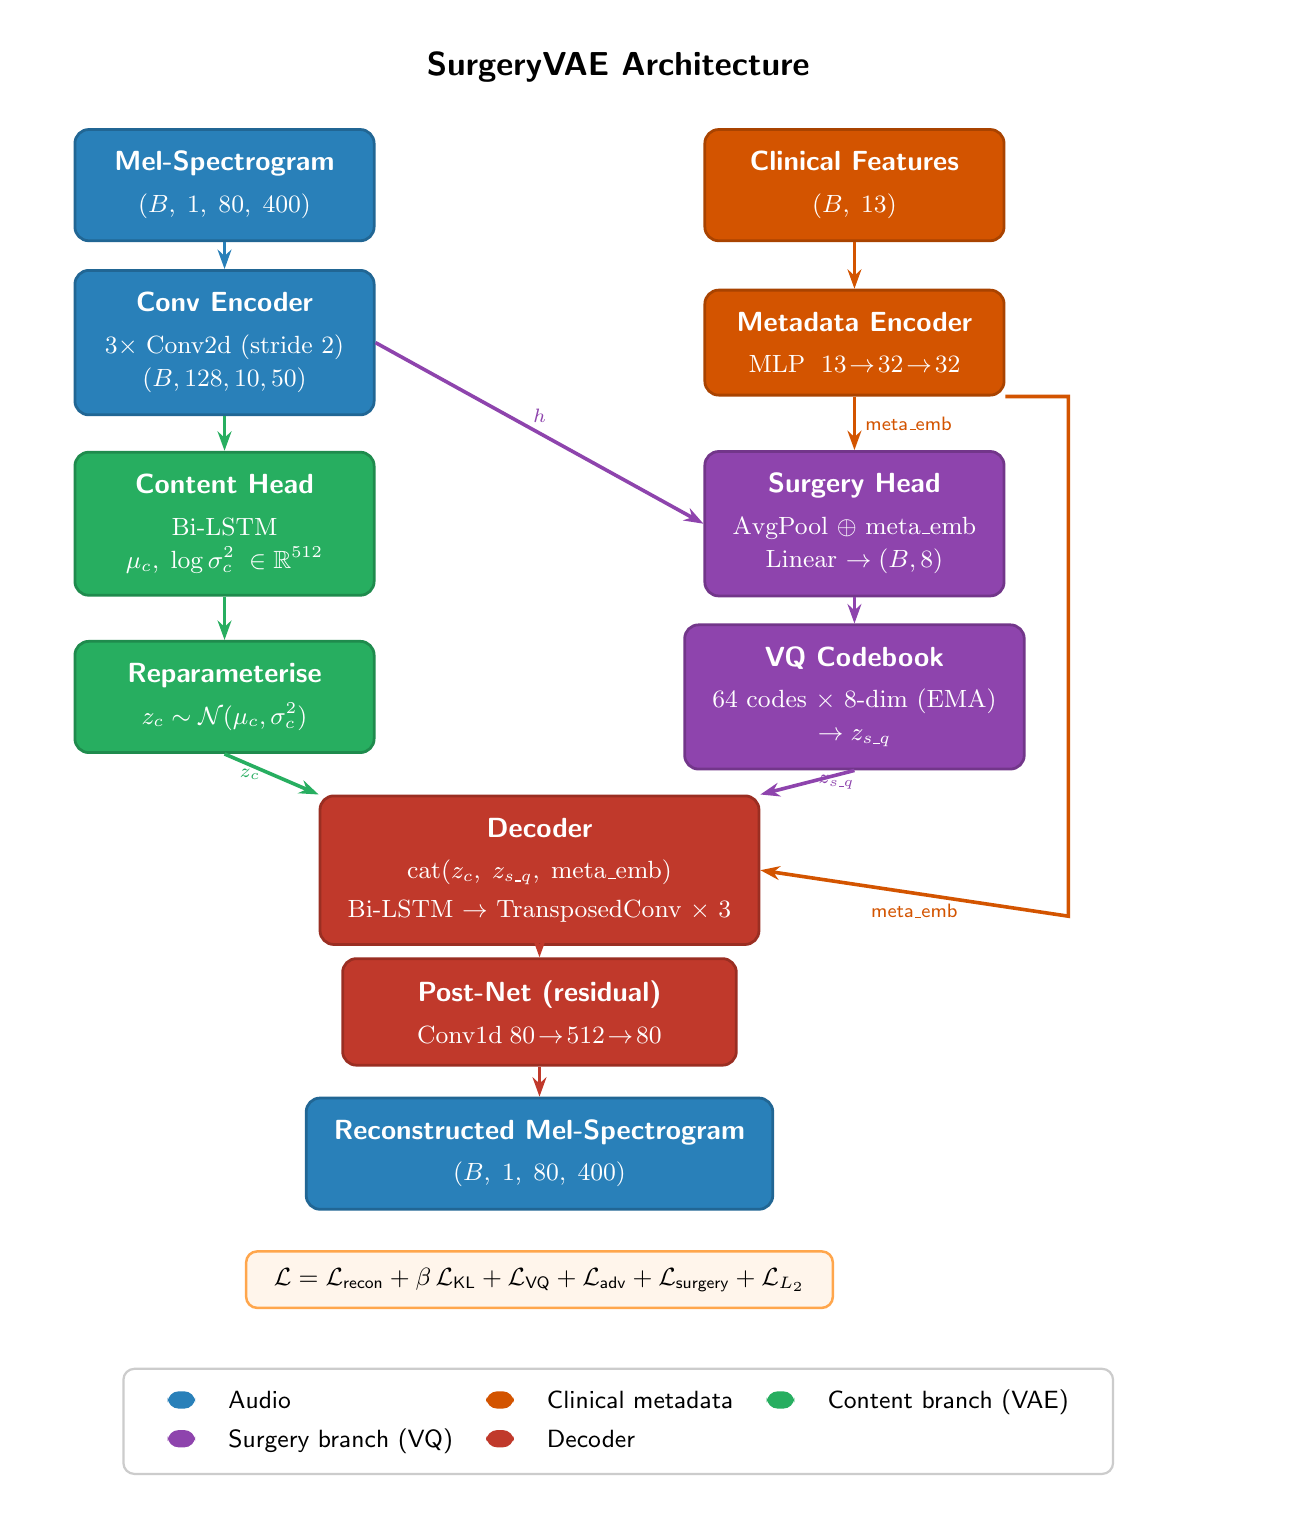
\begin{tikzpicture}[x=1cm, y=1cm]

% ── grid constants ────────────────────────────────────────────────────────────
% columns:  xL=left branch, xR=right branch, xC=centre
\newcommand{\xL}{2}
\newcommand{\xR}{10}
\newcommand{\xC}{6}
\newcommand{\bw}{3.8}   % branch box width
\newcommand{\cw}{5.0}   % centre box width

% ── BACKGROUND ───────────────────────────────────────────────────────────────
\begin{scope}[on background layer]
  \fill[cBg, rounded corners=8pt] (-0.5,-5.0) rectangle (15.5,13.5);
\end{scope}

% ── TITLE ────────────────────────────────────────────────────────────────────
\node[font=\sffamily\large\bfseries] at (7, 13.0)
  {SurgeryVAE Architecture};

% ════════════════════════════════════════════════════════════════════════════
% ROW 1  –  INPUTS  (y = 11.5)
% ════════════════════════════════════════════════════════════════════════════
\node[hdr=cAudio,   minimum width=\bw cm] (mel)  at (\xL, 11.5)
  {Mel-Spectrogram\\[3pt]
   \normalfont\small$(B,\;1,\;80,\;400)$};

\node[hdr=cClinical, minimum width=\bw cm] (clin) at (\xR, 11.5)
  {Clinical Features\\[3pt]
   \normalfont\small$(B,\;13)$};

% ════════════════════════════════════════════════════════════════════════════
% ROW 2  –  ENCODERS  (y = 9.5)
% ════════════════════════════════════════════════════════════════════════════
\node[hdr=cAudio, minimum width=\bw cm] (conv) at (\xL, 9.5)
  {Conv Encoder\\[3pt]
   \normalfont\small 3$\times$ Conv2d (stride 2)\\
   \normalfont\small$(B,128,10,50)$};

\node[hdr=cClinical, minimum width=\bw cm] (metaenc) at (\xR, 9.5)
  {Metadata Encoder\\[3pt]
   \normalfont\small MLP\; $13\!\to\!32\!\to\!32$};

% ════════════════════════════════════════════════════════════════════════════
% ROW 3  –  BRANCH HEADS  (y = 7.2)
% ════════════════════════════════════════════════════════════════════════════
\node[hdr=cContent, minimum width=\bw cm] (chead) at (\xL, 7.2)
  {Content Head\\[3pt]
   \normalfont\small Bi-LSTM\\
   \normalfont\small$\mu_c,\;\log\sigma^2_c\;\in\mathbb{R}^{512}$};

\node[hdr=cSurgery, minimum width=\bw cm] (shead) at (\xR, 7.2)
  {Surgery Head\\[3pt]
   \normalfont\small AvgPool $\oplus$ meta\_emb\\
   \normalfont\small Linear $\to(B,8)$};

% ════════════════════════════════════════════════════════════════════════════
% ROW 4  –  LATENTS  (y = 5.0)
% ════════════════════════════════════════════════════════════════════════════
\node[hdr=cContent, minimum width=\bw cm] (reparam) at (\xL, 5.0)
  {Reparameterise\\[3pt]
   \normalfont\small$z_c\sim\mathcal{N}(\mu_c,\sigma_c^2)$};

\node[hdr=cSurgery, minimum width=\bw cm] (vq) at (\xR, 5.0)
  {VQ Codebook\\[3pt]
   \normalfont\small 64 codes $\times$ 8-dim (EMA)\\
   \normalfont\small$\to z_{s\_q}$};

% ════════════════════════════════════════════════════════════════════════════
% ROW 5  –  DECODER  (y = 2.8)
% ════════════════════════════════════════════════════════════════════════════
\node[hdr=cDecoder, minimum width=\cw cm] (dec) at (\xC, 2.8)
  {Decoder\\[3pt]
   \normalfont\small
   $\text{cat}(z_c,\;z_{s\_q},\;\text{meta\_emb})$\\[2pt]
   \normalfont\small Bi-LSTM $\to$ TransposedConv $\times$ 3};

% ════════════════════════════════════════════════════════════════════════════
% ROW 6  –  POST-NET  (y = 1.0)
% ════════════════════════════════════════════════════════════════════════════
\node[hdr=cDecoder, minimum width=\cw cm] (postnet) at (\xC, 1.0)
  {Post-Net (residual)\\[3pt]
   \normalfont\small Conv1d\;$80\!\to\!512\!\to\!80$};

% ════════════════════════════════════════════════════════════════════════════
% ROW 7  –  OUTPUT  (y = -0.8)
% ════════════════════════════════════════════════════════════════════════════
\node[hdr=cAudio, minimum width=\cw cm] (out) at (\xC, -0.8)
  {Reconstructed Mel-Spectrogram\\[3pt]
   \normalfont\small$(B,\;1,\;80,\;400)$};

% ════════════════════════════════════════════════════════════════════════════
% ARROWS
% ════════════════════════════════════════════════════════════════════════════

% -- inputs to encoders (straight down) --
\draw[arr=cAudio]    (mel)     -- (conv);
\draw[arr=cClinical] (clin)    -- (metaenc);

% -- conv to content head (straight down) --
\draw[arr=cContent]  (conv)    -- (chead);

% -- conv to surgery head (diagonal right) --
\draw[arr=cSurgery]  (conv.east) -- node[above, font=\sffamily\scriptsize,
                                          text=cSurgery, pos=0.5]{$h$}
                     (shead.west);

% -- meta encoder to surgery head (straight down) --
\draw[arr=cClinical] (metaenc) -- node[right, font=\sffamily\scriptsize,
                                        text=cClinical]{meta\_emb}
                     (shead);

% -- content head to reparameterise (straight down) --
\draw[arr=cContent]  (chead)   -- (reparam);

% -- surgery head to VQ (straight down) --
\draw[arr=cSurgery]  (shead)   -- (vq);

% -- reparameterise to decoder (diagonal to centre) --
\draw[arr=cContent]  (reparam.south) -- node[left, font=\sffamily\scriptsize,
                                              text=cContent]{$z_c$}
                     (dec.north west);

% -- VQ to decoder (diagonal to centre) --
\draw[arr=cSurgery]  (vq.south) -- node[right, font=\sffamily\scriptsize,
                                         text=cSurgery]{$z_{s\_q}$}
                     (dec.north east);

% -- meta to decoder  (right-side vertical bypass) --
\draw[arr=cClinical]
  (metaenc.south east) -- ++(0.8,0) -- ++(0,-6.6)
  -- node[below, font=\sffamily\scriptsize, text=cClinical]{meta\_emb}
  (dec.east);

% -- decoder to post-net to output --
\draw[arr=cDecoder]  (dec)     -- (postnet);
\draw[arr=cDecoder]  (postnet) -- (out);

% ════════════════════════════════════════════════════════════════════════════
% LOSS BOX  (below output)
% ════════════════════════════════════════════════════════════════════════════
\node[draw=orange!70, fill=orange!8, rounded corners=4pt,
      font=\sffamily\small, align=center, line width=0.9pt,
      inner xsep=10pt, inner ysep=6pt] at (\xC, -2.4)
  {$\mathcal{L}=
     \mathcal{L}_{\text{recon}}
    +\beta\,\mathcal{L}_{\text{KL}}
    +\mathcal{L}_{\text{VQ}}
    +\mathcal{L}_{\text{adv}}
    +\mathcal{L}_{\text{surgery}}
    +\mathcal{L}_{L_2}$};

% ════════════════════════════════════════════════════════════════════════════
% LEGEND  (bottom, horizontal)
% ════════════════════════════════════════════════════════════════════════════
\newcommand{\lsq}[1]{%
  \tikz{\fill[#1] (0,0) rectangle (0.35,0.22);}}

\node[draw=black!20, fill=white, rounded corners=4pt, line width=0.8pt,
      inner xsep=10pt, inner ysep=6pt] at (7, -4.2) {
  \begin{tabular}{cl@{\hspace{12pt}}cl@{\hspace{12pt}}cl}
    \lsq{cAudio}    & \sffamily\small Audio &
    \lsq{cClinical} & \sffamily\small Clinical metadata &
    \lsq{cContent}  & \sffamily\small Content branch (VAE) \\[2pt]
    \lsq{cSurgery}  & \sffamily\small Surgery branch (VQ) &
    \lsq{cDecoder}  & \sffamily\small Decoder &
                    & \\
  \end{tabular}};

\end{tikzpicture}
\end{document}
